%===============================================================================
%===============================================================================
%
\clearpage
%
\subsection{Example-0004 \texttt{[VALIDATED]}}
%
Example uses generated regular meshes and solves a static problem, i.e., applies
the boundary conditions in one step.
%
%===============================================================================
%
\subsubsection{Mathematical model - 2D}
%
We solve the following scalar equation,
%
\begin{align}
    \nabla \cdot \nabla u = 0 & &&\Omega = [0, 2] \times [0, 1],
\end{align}
%
with boundary conditions
%
\begin{align}
    u = 2.0 e^x \cdot cos(y)    & &&\text{on } \partial\Omega.
\end{align}
%
No material parameters to specify.
%
%===============================================================================
%
\subsubsection{Computational model}
%
\begin{itemize}
    \item{Commandline arguments are:}
        \subitem{integer: number of elements in x-direction}
        \subitem{integer: number of elements in y-direction}
        \subitem{integer: number of elements in z-direction (set to zero for 2D)}
        \subitem{interger: interpolation order (1: linear; 2: quadratic)}
        \subitem{integer: solver type (0: direct; 1: iterative)}
    \item{Commandline arguments for tests are:}
        \subitem{4 2 0 1 0}
        \subitem{8 4 0 1 0}
        \subitem{2 1 0 2 0}
        \subitem{4 2 0 2 0}
        \subitem{8 4 0 2 0}
        \subitem{4 2 0 1 1}
        \subitem{8 4 0 1 1}
        \subitem{2 1 0 2 1}
        \subitem{4 2 0 2 1}
        \subitem{8 4 0 2 1}
        \subitem{100 50 0 1 0 (not tested yet..)}
        \subitem{100 50 0 2 0 (not tested yet..)}
        \subitem{100 50 0 1 1 (not tested yet..)}
        \subitem{100 50 0 2 1 (not tested yet..)}
\end{itemize}
%
%===============================================================================
%
\subsubsection{Result summary}
%
We use CHeart rev.\ 6292 to produce numerical reference solutions.
%
\verbatiminput{examples/example-0004/results/results.summary}
\verbatiminput{examples/example-0004/results/failed.tests}
%
\begin{figure}[h!]
    \centering 
    \includegraphics[width=0.9\columnwidth]{examples/example-0004/doc/figures/iron_reference_2D.eps} 
    \caption{2D results, iron reference w/ command line arguments [8 4 0 2 0].}
    \label{example-0004-iron-2D-reference-fig}
\end{figure}
%
\begin{figure}[h!]
    \centering 
    \includegraphics[width=0.9\columnwidth]{examples/example-0004/doc/figures/current_run_l4x2x0_n8x4x0_i2_s0.eps} 
    \caption{2D results, current run w/ command line arguments [8 4 0 2 0].}
    \label{example-0004-current-run-2D-fig}
\end{figure}
%
%===============================================================================
%===============================================================================
